\section{Method}
\label{sec:method}

\begin{figure}[t]
\centering
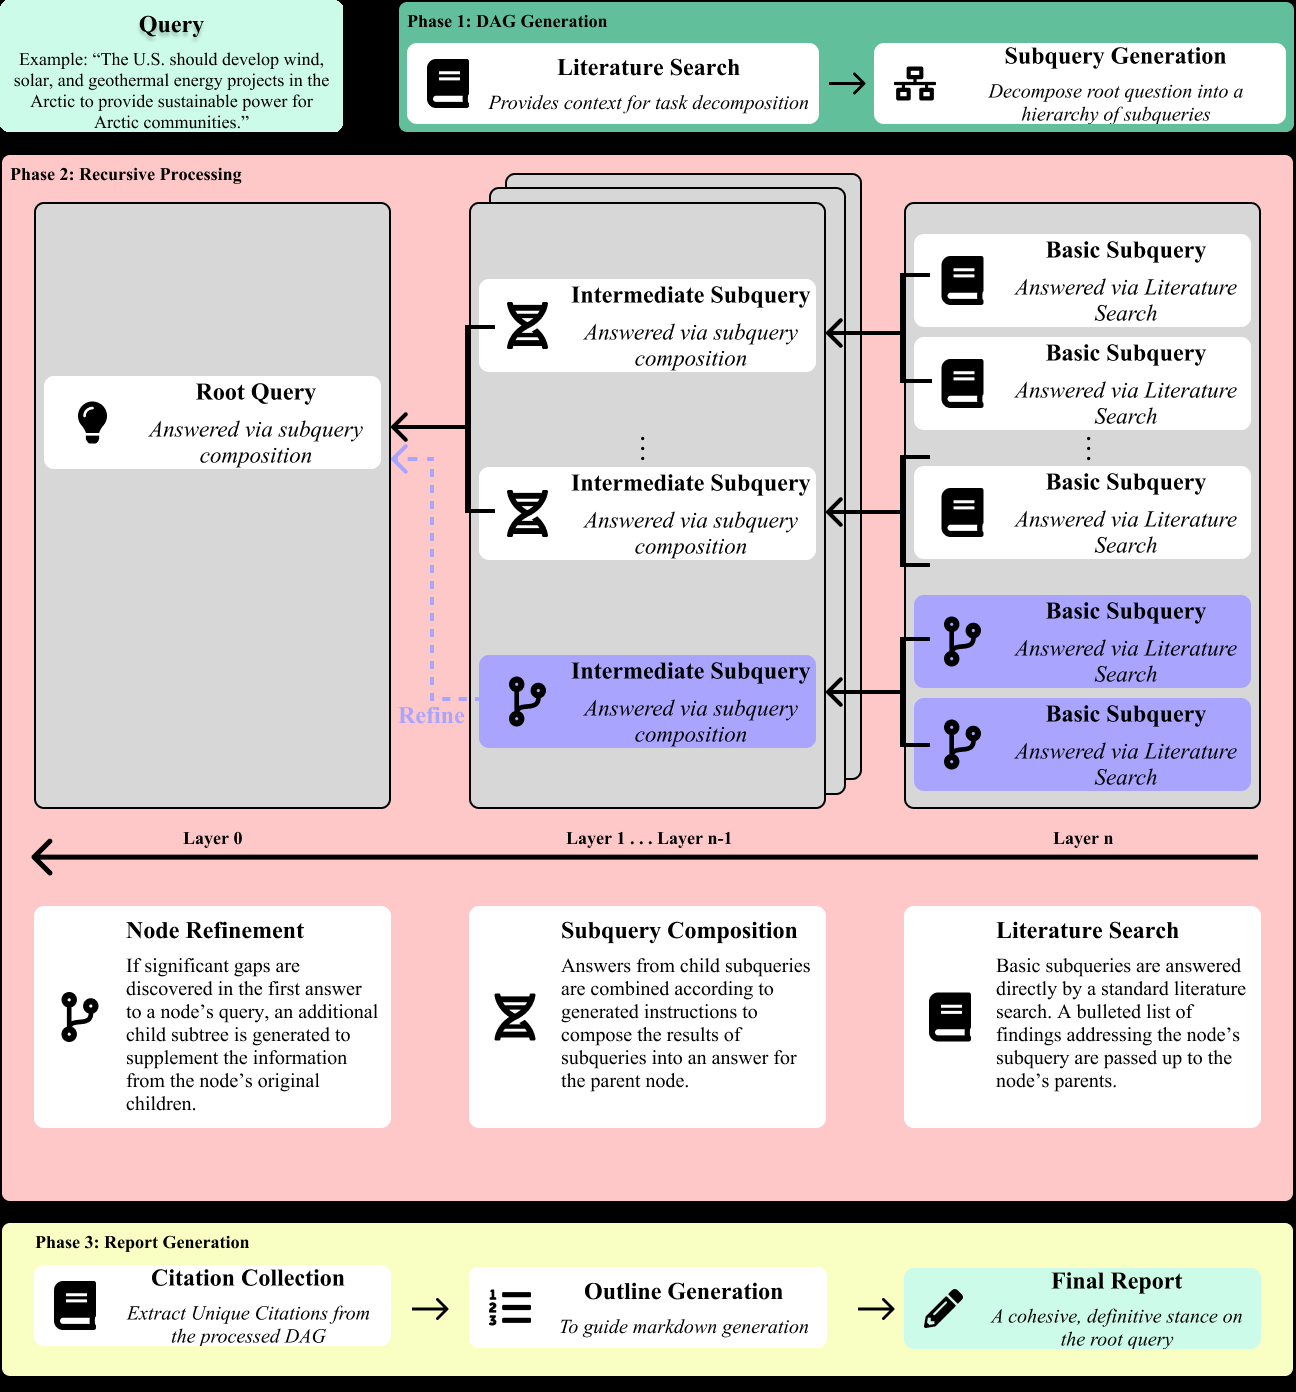
\includegraphics[width=\linewidth]{figs/pipeline.png}
\caption{The three phases of \sys{}. In Phase 1, a literature search is used to contextualize the question and decompose it into a DAG of sub-questions. In Phase 2, leaves are answered using literature search, parents are composed from their children, and then the pipeline iterates to refine nodes with incomplete answers by adding new sub-trees. In Phase 3, the fully completed DAG is converted into an outline and a report that justifies the root answer.}
\label{fig:pipeline}
\end{figure}

\sys{} takes a research question as input and returns a report that is properly citation-backed and advances an answer to the question. It works in three phases: DAG creation, recursive answering, and report crafting. This section describes the pipeline version used to generate the reports in \Cref{sec:experiments}; code versions are listed in \Cref{app:changes}. All calls to language models in the pipeline are made using DSPy signatures \citep{khattab2024dspy} (details in \Cref{app:prompts}).

\paragraph{Literature search.}
The planning phase and leaf nodes both use the same literature search process. First, a planning model generates web search queries from the question. A retriever uses the Serper API to fetch results and extract page content, and then uses \texttt{text-embedding-3-large} to embed all passages and select the most relevant ones for the query. An answer model then answers the query with citations from the passages. After each iteration, a completion model decides if another round of search is necessary, limited by a maximum number of retriever calls per question.

\paragraph{Phase 1: DAG generation.}
To begin, a brief literature search is done on the main question to provide context. Then, the planning model creates the DAG layer-by-layer, asking child sub-questions from every node in the current layer. For each node, the model uses the node's question, the literature search summary, the children nodes created so far, and the entire graph structure to create the children. Using the entire graph prevents duplicate sibling questions and encourages the children of a node to jointly address the question. There are limits placed on the depth of the graph, the number of nodes, and the number of children per node.

Another pass generates composition instructions for every parent. These instructions are based on the parent's question, the parent's desired output format, and the children's questions. The model is asked to explain how the children's answers can be combined to generate an answer for the parent. The instructions use unique identifiers for children to make all the dependencies clear.

\paragraph{Phase 2: recursive answering.}
The DAG is topologically sorted, and then processed bottom-up, since parents are composed from answered children. Leaves are answered in parallel using literature search, with the answer model generating bullet points using the desired format while preserving all citations. Then parents are composed in topological order. The synthesis model uses the children's answers, the composition instructions, and the desired output format to generate the parent's answer. The model is asked to use only text from the children's answers and use the same citation numbers from the children's answers. Additionally, the model must indicate any contradictory claims between children. Since parents only depend on children, any citation made in the parent's answer should trace back to evidence gathered at a leaf.

\paragraph{Gap exploration and refinement.}
It is possible that the initial plan will miss something that the research later shows to matter. Thus, after composing a parent, a gap explorer identifies any potential gaps in the answer. A gap evaluator then evaluates if the gap is important, at a configurable conservatism level. If it is, a new sub-tree is generated of questions addressing the gap, and then attached under the parent. The new sub-tree is processed in the same way as the rest of the graph, and the parent is re-composed. In our current setup, a parent will only see one pass of this refinement.

\paragraph{Phase 3: report generation.}
After the DAG is completed, it is converted to text, and all citations are unified to a single list of numbered citations. Next, the report is outlined and generated. An outline model is asked to advocate for a position on the root question, and then generates an outline where each section maps to each branch in the graph. Then, the report is generated using the outline and the graph. The model is asked to use the same citations, advocate for the root answer's claim, and name the report the claim rather than the question. Finally, the pipeline standardizes the numbering and adds a bibliography.

\begin{algorithm}[t]
\caption{\sys{}}
\label{alg:pipeline}
\begin{algorithmic}[1]
\Require motion $m$, limits on depth $d$, nodes $n$, and children $c$, refinement rounds $\rho$
\State $L \gets \textsc{LiteratureSearch}(m)$ \Comment{context for planning}
\State $G \gets$ root $r$ with $q_r = m$
\For{each layer $\ell = 0, \dots, d-1$} \Comment{Phase 1}
  \For{each node $u$ at depth $\ell$}
    \State add children $\textsc{PlanChildren}(q_u, L, G, c)$ under $u$, within the node limit $n$
  \EndFor
\EndFor
\For{each parent $u$} $\kappa_u \gets \textsc{CompositionInstructions}(q_u, \{q_v : v \in C(u)\})$ \EndFor
\For{each node $u$ in topological order, leaves first} \Comment{Phase 2}
  \If{$u$ is a leaf}
    \State $(a_u, S_u) \gets \textsc{AnswerFromSearch}(q_u)$
  \Else
    \For{$k = 0, \dots, \rho$}
      \State $a_u \gets \textsc{Compose}(q_u, \{a_v\}_{v \in C(u)}, \kappa_u)$, \quad $S_u \gets \bigcup_{v \in C(u)} S_v$
      \State $\Delta \gets \textsc{FindGaps}(q_u, a_u)$
      \If{$k = \rho$ \textbf{or} $\Delta = \emptyset$} \textbf{break} \EndIf
      \State attach a sub-tree for $\Delta$ under $u$ and process it as in Phase 2
    \EndFor
  \EndIf
\EndFor
\State $O \gets \textsc{Outline}(m, a_r, G)$, \quad $R \gets \textsc{Report}(O, m, a_r, G)$ \Comment{Phase 3}
\State \Return $R$ with a bibliography of $\bigcup_v S_v$
\end{algorithmic}
\end{algorithm}

Let $|V_\text{leaf}|$ be the number of leaves in the finalized DAG, and let $|V_\text{par}|$ be the number of parent nodes. Each leaf node makes $1$ literature search call, which includes generating a search query, retrieving with embedding, making an answer call, and checking completeness. Each parent node makes $1$ composition call per refinement round, and $1$ gap check. For planning, each parent node makes $1$ planning call to plan the children, and $1$ planning call for instructions. Additionally, writing has $2$ calls. Overall, the total approximate number of model calls is $4|V_\text{leaf}| + (3+2\rho)|V_\text{par}| + 3$. This means the total number of calls is linear in the size of the graph. We can call literature searches for leaves in parallel (\Cref{alg:pipeline}). In \Cref{app:dag}, we provide an example run of the logged experiment, which has \dagLeaves{} leaves and \dagParents{} parent nodes. The system uses about $40$ model calls, which is much more than the $1$ or a few calls needed for the standard one-pass report.

For evaluations we use GPT-4.1-mini for all retrieval-based answers and planning, GPT-5 for DAG generation, synthesis, and report writing, and \texttt{text-embedding-3-large} for retrieval. All models are accessed through Azure OpenAI. By default, we set a maximum DAG depth of 2 and a maximum number of 50 nodes. To keep the DAG sparse, we also limit the number of children per node to 10. We use $1$ retriever call per literature search and $1$ refinement round per parent by default.
